\documentclass[Main]{subfiles}

\begin{document}
\chapter{Lagrangian Systems and Pierels Brackets}
   %introduzione
	\danger .. introduzione

	\section{Abstract Mechanical Systems}
	It's possible to state a mathematical definition sufficiently broad to include all the systems in ordinary analytical mechanics regardless of the cardinality of degrees of freedom  in a unified way.
	
	\begin{definition}[Abstract Evolutive System]
		Pair $(E,P )$ composed of:
		\begin{itemize}
			\item $E \xrightarrow{\pi} M$ \\smooth fiber bundle of typical fiber $Q$ on  manifold $M$ called \emph{"configuration bundle"}.
			\item	$ P : \Gamma^\infty(E) \rightarrow \Gamma^\infty(E)$ \\  operator called \emph{"motion operator"}
		\end{itemize}
	\end{definition}
	This formultation is still very distant from the physical interpretation but has the benift to highlight the minimal mathematical objects which must be fixed in order to specify a mechanical systems.
	
	
	\paragraph{Kinematics}
	%Fibrato Configurazione incompassa la cinematica
	The configuration bundle encompass all the kinematical structure of the system, the pivotal role is played by the smooth sections  which are to be understood as all the possible conformation of the system.

	\begin{notationfix}
		\begin{displaymath}
			\Conf \coloneqq \Gamma^\infty(M,E)
		\end{displaymath}
		Space of kinematic configurations.
	\end{notationfix}

	A section is not a statical configuration, equivalent to a specific point in the configuration space of ordinary classical systems, but has to be seen as a specific realization of the kinematics in the sense of  a complete description of a possible motion.
	At this level of abstraction, since no space-time structure has been specified, terms like stasis and motion must be taken with care .The natural physical interpretation should be clearly manifested through the concrete realization of systems with discrete and continuous degree of freedom.
	
	\begin{observation}[Mathematical structure]
	Mathematically speaking this set should be regarded as an infinite dimensional Manifold. 
	\\
	This framework provides a geometric characterization of the notion of variations as tangent vectors on the the space of kinematic configurations .\cite{Forger2005}
	\end{observation}
	
	\begin{observation}[Coordinate Representation]
	The choice of a chart atlas $\Atlas(M)$ on the base space $M$ and $\Atlas(E)$ on the total space $E$ provides a correspondence between each configuration $\gamma \in \Conf$ and family of smooth real functions $\{f_{\alpha \beta}:A_\alpha \subset \Real^m \rightarrow \Real^q \}$.
	The process is trivial:
	\begin{displaymath}
		\gamma \in \Conf \mapsto \{f_{A,U}=\psi_U \circ \gamma \circ \psi_A^{-1} \vert (A,\psi_A) \in \Atlas(M), (U,\psi_U)\in \Atlas(E)   \}
	\end{displaymath}
	
	%	$\forall (A,\psi_A)$ local chart on $M$ and $(U,\psi_U)$ local chart on $E$ such that $\gamma(A) \cap U \neq \emptyset$ $f_{A,U}=\psi_U \circ \gamma \circ \psi_A^{-1}$

	Since the whole section as a global object is quite difficult to handle is customary in field theory to work in the more practical local representation. 
	\end{observation}	
	
	\begin{observation}[Further specification of the system's kinematics]
	 	The general formalism doesn't require any other structure to be carried forward.
	 	Additional structure on the fiber , the base or the whole bundle are to be prescribed in order to specify a precise physical model, e.g. the spin structure on $E$ for the Dirac Field.\cite{Benini}
	 \end{observation}	
	
	\paragraph{Dynamics}
	The operator $P$ is the object that contains all the information about the dynamic evolution of the system.
	It has the role to select the dinamically compatible configuration among all the admissible kinematic configurations of $\Conf$, exactly as it happens in analytical mechanics where the dynamic equations shape the natural motions.
	\begin{notationfix}
		Provided an equations of motion operator
		\begin{displaymath}
			P: \Conf \rightarrow \Conf
		\end{displaymath}
		The space
		\begin{displaymath}
		\Sol \coloneqq \ker(P) \subset \Conf
		\end{displaymath}
		is called \emph{"Space of Dynamical Configurations"}.
	\end{notationfix}
	
	\begin{figure}[h!]
 	 	\caption{Geometric picture of the basic mechanical system's structure.}
 	 	\danger immagine
   		%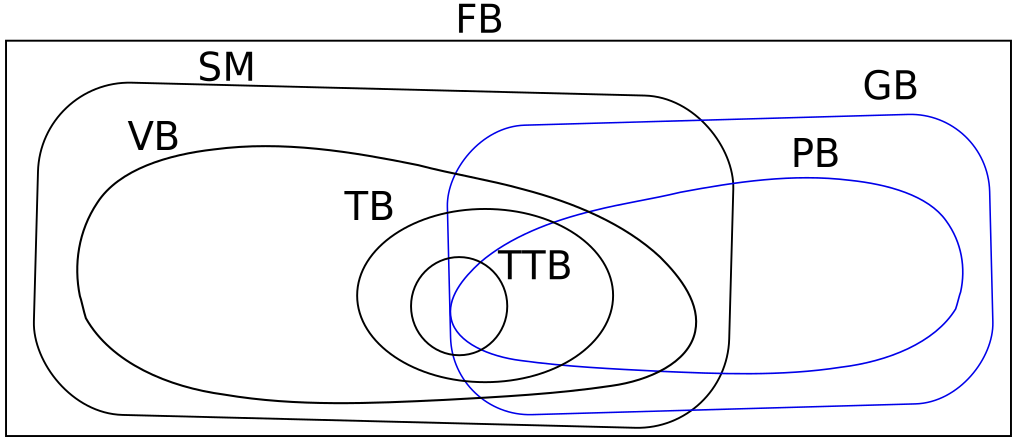
\includegraphics[width=0.5\textwidth]{Pictures/EuleroVenn_Bundles} 
  		\centering
	\end{figure}	
	
	\subsection{Lagrangian Dynamics}	
	Lagrangian systems constitute a subclass of the abstact mechanical systems of more practical interest:	
		\begin{definition}[Lagrangian System]
	Pair $(E, \mathcal{L} )$ composed of:
		\begin{itemize}
			\item $E \xrightarrow{\pi} M$ \\smooth fiber bundle of typical fiber $Q$ on the oriented manifold $(M,\mathfrak{o})$ called \emph{"configuration bundle"}.
			\item	$ \Lagrangian : J^r E \rightarrow \wedge^m T^*M$ \\bundle-morphism from the r-th Jet Bundle to  the top-dimensionial forms bundle over the base manifold $M$  called \emph{"Lagrangian density"} or simply \emph{"Lagrangian"} of r-th order.
		\end{itemize}
	\end{definition}	
	In what follows all the systems considered will be exclusively of first order.
	
	
	%la lagrangiana incompassa la dinamica
	In this case is the Lagrangian density the object containing all the information about the dynamic evolution of the system.

	%In Layman terms la lagrangiana  è un qualcosa che può essere integrato sopra la varietà
	In order to reconstruct the system's dynamic from the Lagrangian density has to be understood the mathematical nature of $\Lagrangian$.
	$\Lagrangian$ maps point $q_p$ on the fiber $J^r_p E$ to a m-form on $T_p M$.
	Recalling the definition of jet bundles is clear that for each smooth section on $E$ is associated a smooth section on the b$J^rE$ :
	\begin{displaymath}
		\phi \in \Gamma^\infty (E) \mapsto (\phi, \partial_\mu \phi, \partial_{\mu, \nu} \phi , \ldots \partial_{\vec{\alpha}}\phi)
	\end{displaymath}
	where  $\vec{\alpha}$ is a multi-index of length r.
	The correspondence is not univocal since sections equal up to the r-th order define the same jet section.
	The smoothness of $\Lagrangian$ ensure that each jet bundle section is mapped to a smooth section in the top-forms bundle i.e. the most general integrable object on a orientable manifold.
	
	%la classe delle densità lagrangiane
	It should be clear that $\Lagrangian$ is a specific choice among the vast class of functions suitable to be a good Lagrangian density over the  Configuration Bundle $E$:
	\begin{definition}[Lagrangian Density on the bundle $E$]
		\begin{displaymath}
			\Lag^r (E) \coloneqq \hom\biggr(J^r E,\quad \bigwedge^m( T^*M)\biggr)  \cong \big\{f:\Gamma^\infty(J^r E) \rightarrow \Omega^m(M)  \big\}
		\end{displaymath}
	(where $\Omega^m(M)$ is the common name for $\Gamma^\infty \big( \bigwedge^m( T^*M) \big)$ in the context of Grassmann algebras.)
	The equivalence states the fact that a bundle-morphism induce a mapping between the sections.
	\end{definition}
	 this choice fix the "Dynamical identity" of the considered system.
	\begin{proposition}
		$\Lag^r(E)$ has an obvious vector space structure inherited by the linear structure of $\Omega(M)$.
	\end{proposition}
	
	
	Thanks to the correspondence between a section $\phi \in \Conf$ and his r-th jet, it's possible to consider the Lagrangian as directly acting on the kinematic configurations.
	The image  $\Lagrangian [ \phi ] \textrm{d}\mu$ , where $\textrm{d}\mu$ is the measure associated to the orientation $\mathfrak{o}$, is an object that can be measured on the whole base space, this property suggests the introduction of a class of associated functionals:
	\begin{definition}[Lagrangian functional]
		Is a functional on $\Conf$ with values on regular distribution over M associated to the generic $\Lagrangian \in \Lag$.	
		\begin{displaymath}
			\mathcal{O}_\Lagrangian : \Conf \rightarrow \big( C^\infty_0(M) \big)'
		\end{displaymath}			
			Such that the lagrangian functional associated to $\Lagrangian$, valued on the configuration $\phi \in \Conf$ and tested on the test-function $f \in C^\infty_0(M)$ it's given by:
		\begin{displaymath}
			\mathcal{O}_\Lagrangian [\phi] (f) = \int_M \Lagrangian [\phi] f \textrm{d}\mu
		\end{displaymath}		
	\end{definition}	
	
	\begin{proposition}
		As a distribution $\mathcal{O}_\Lagrangian [\phi] (f) $ is necessarily linear in the test-functions entry but not in the configurations entry.	
	\end{proposition}	
	
	\begin{observation}
		The choice of the image of $\mathcal{O}_\Lagrangian$ as a distribution it's a necessary precaution to ensure that functional is \emph{"convergent"} whatever is the configuration on which is evaluated.
		In fact, despite $\Lagrangian [ \phi ]$ is integrable with respect to the measure $\textrm{d}\mu$, it's not necessary summable if the support of the configuration $\phi$ becomes arbitrarily large.
		\\
		This is a simple consequence of the well known sequence of inclusions:
		\begin{displaymath}
			\Lagrangian [ \phi ] \in C^\infty_0(M) \subset L^1_{\textrm{loc}}(M,\mu) \supsetneqq  L^1(M,\mu) 
		\end{displaymath}
		of the functional analysis .
		Indeed, the functional
		\begin{displaymath}
			\mathcal{O}_\Lagrangian [\phi]= \int_{\supp(\phi)} \Lagrangian [\phi] \textrm{d}\mu
		\end{displaymath}
		is well defined for all $\Lagrangian \in \Lag^r(E)$ only over the compactly supported sections. 
		To take account of the global sections it's sufficient to dampen the integral multiplying the integrand with an arbitrary test-function.
	%il funzionale lagrangiana totale e azione
	\end{observation}
	
	\begin{notationfix}
		When calculated for the specific density of the Lagrangian system $\mathcal{O}_\Lagrangian$ takes the name of \emph{Action} or \emph{Total Lagrangian}. 
	\end{notationfix}

	The introduction of the Lagrangian density is meaningless without the prescription of a dynamical principle which allows to determine univocally a differential operator $P$ on the kinematics configurations space $\Conf$.
	This fundamental principle is the \emph{least action principle}.
	A proper justification of this claim should require the presentation of the differential calculus on the infinite dimensional manifolds $\Conf$. 
	Jumping straight to the conclusion we can state this correspondence as a principle  in term of a function which assign for all lagrangian densities an operator on the kinematic configurations space. In the case of first order lagrangian we define
	\begin{definition}[Euler-Lagrange operator]
		It's the differential operator
		\begin{displaymath}
			Q_\chi : \Conf \rightarrow \Conf
		\end{displaymath}
		relative to the lagrangian density $\chi \in \Lag^1(E)$, such that:
		\begin{equation}
			Q_\chi (\gamma) = \Biggr( \partial_\mu \biggr( \frac{\partial \chi}{\partial(\partial_\mu \phi)} \biggr\vert_\gamma \biggr) - \frac{\partial \chi}{\partial \phi}\biggr\vert_\gamma \Biggr) \qquad \forall \gamma \in \Conf
		\end{equation}
		(where 	$\biggr( \frac{\partial \chi}{\partial(\partial_\mu \phi)}$ is the be intended as the lagrangian density constructed differentiating $\chi(\phi, \partial_\mu)$ as an ordinary function treating its functional entries as an usual scalar variable.)
	\end{definition}

	
	\begin{observation}
		The whole theory of both Lagrangian densities class and Euler-Lagrange equation could be stated in a more syntetic way in terms of the Grassmann-graded variational bicomplex.\cite{Giachetta2009}\cite{Sardanashvily}
	\end{observation}
	
		

	
%-_-_-_-_-_-_-_-_-_-_-_-_-_-_-_-_-_-_-_-_-_-_-_-_-_-_-_-_-_-_-_-_-_-_-_-_-_-_-_-_-_-_-_-_-_-_-_-_-_-_-_-_-_-_-_
\newpage
	\section{Concrete Realization}
	%esibiamo quanto è ampia la nostra definizione
		\subsection{Fields on curved Background}
		M è spazio tempo,
		bundle è lineare per prevedere il principio di sovrapposizione
		M è glob iper e P è green iper per tener conto del comporatamento propagativo
		definire sup cauchy
		definire s-t iperbolico (solo la caratterizzazione di ammetre una sup di cauchy)
		definire op green iperbolico su spazio tempo iperbolico (cioè ha delle green ope)
		Propr di buona definizione esistenza e unicita della soluzione
		
		Di particolare ricorrenza fisica sono gli operatori normally iperbolic
		espressione in coordinate
		esempio K-g!

		\subsection{Finite Degree systems}
		  % il fibrato non è vettoriale
		  % le configurazioni sono curve
		  % 
		
%-_-_-_-_-_-_-_-_-_-_-_-_-_-_-_-_-_-_-_-_-_-_-_-_-_-_-_-_-_-_-_-_-_-_-_-_-_-_-_-_-_-_-_-_-_-_-_-_-_-_-_-_-_-_-_
\newpage
	\section{Geometric mechanics of Finite Degree systems}
	%L'approccio usato generalmente è deduttivo dal particolare al generale
	%parlare di spazio delle fasi, forma simplettica, legendre
	%osservabili classici parentesi di poisson
	
	\subsection{Linear dynamical systems}	
	
%-_-_-_-_-_-_-_-_-_-_-_-_-_-_-_-_-_-_-_-_-_-_-_-_-_-_-_-_-_-_-_-_-_-_-_-_-_-_-_-_-_-_-_-_-_-_-_-_-_-_-_-_-_-_-_
\newpage
	\section{Peierls Brackets}
	%peierels vs poisson (sharan)
	
	\subsection{Finite Dimensional case}
	
%-_-_-_-_-_-_-_-_-_-_-_-_-_-_-_-_-_-_-_-_-_-_-_-_-_-_-_-_-_-_-_-_-_-_-_-_-_-_-_-_-_-_-_-_-_-_-_-_-_-_-_-_-_-_-_
\newpage
	\section{Eliminata}
	\begin{itemize}
		\item quando parlo della cinematica mi piacerebbe dare indicazioni sulla struttura matematica dello spazio delle configurazioni cinematiche:
			\begin{enumerate}
				\item costituisce una frechet manifold ( gli unici risultati che ho trovato sono quelli di Palais di "non linear global analysis"
				\item le curve parametrizzate sono le variazioni
				\item classi di equivalenza definiscono delle variazioni infinitesime che costituiscono lo spazio tangente allo spazio delle configurazioni cinematiche
				\item questo spazio tangente è isomorfo allo spazio delle sezioni del pullback rispetto alla sezione $\phi\in C$ del verical bundle (vedere forger romero)
				\item il problema dell'atlante e della rappresentazione delle sezioni in carta locale ( da scegliere sia sul total space E che sul base space M)
			\end{enumerate}
	\end{itemize}
	
\end{document}